\documentclass{minimal}
\usepackage[paperwidth=6.1in,paperheight=2.75in,margin=0.05in]{geometry}
%\usepackage[paperwidth=6.1in,paperheight=3.53in,margin=0.05in]{geometry}

\usepackage[utf8]{inputenc}
\usepackage{amsmath}
\usepackage{amsfonts}
\usepackage{amssymb}

\usepackage{tikz}

%\usetikzlibrary{shapes.geometric, arrows}
%\tikzstyle{startstop} = [rectangle, rounded corners, minimum width=3cm, minimum height=1cm,text centered, draw=black, fill=red!30]
%\tikzstyle{process} = [rectangle, minimum width=2cm, minimum height=1cm, text centered, draw=black, fill=orange!30]
%\tikzstyle{process_2} = [rectangle, minimum width=2cm, minimum height=1cm, text centered, text width=4cm, draw=black, fill=orange!30]
%\tikzstyle{process_3} = [rectangle, minimum width=2cm, minimum height=1cm, text centered, text width=2cm, draw=black, fill=orange!30]
%\tikzstyle{arrow} = [thick,->,>=stealth]

%\usetikzlibrary{matrix,chains,positioning,decorations.pathreplacing,arrows}
\usetikzlibrary{decorations.pathreplacing}


\begin{document}
\def\layersep{2.0cm}
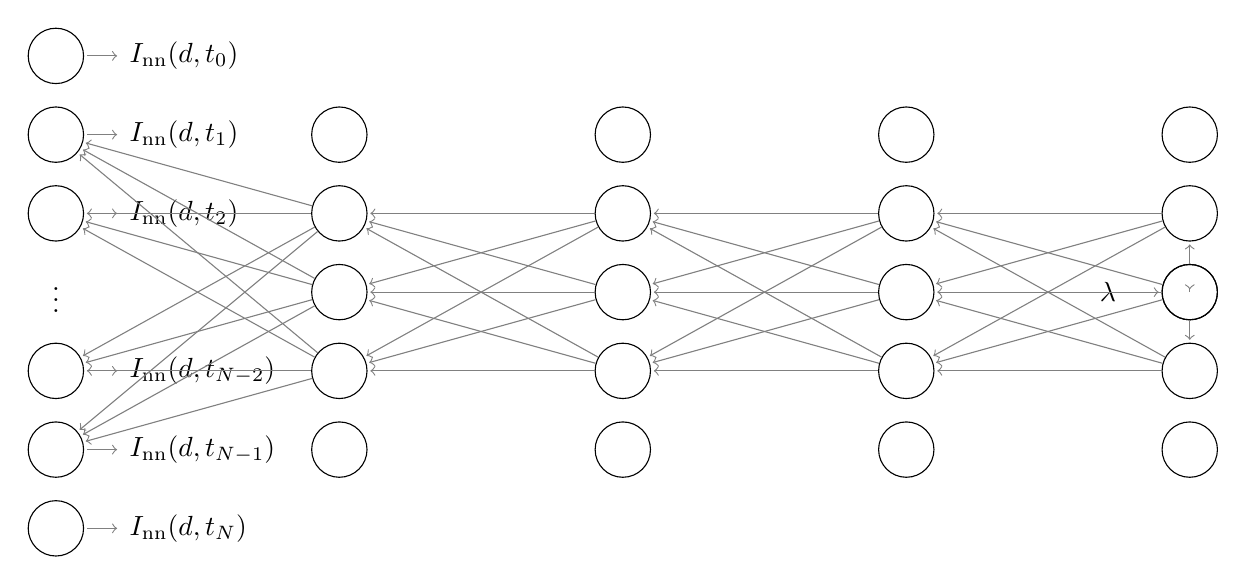
\begin{tikzpicture}[shorten >=1pt,->,draw=black!50, node distance=\layersep]
    \tikzstyle{every pin edge}=[<-,shorten <=1pt]
    \tikzstyle{neuron}=[circle,draw=black,minimum size=20pt,inner sep=0pt]
    \tikzstyle{input neuron}=[neuron, fill=green!50];
    \tikzstyle{output neuron}=[neuron, fill=red!50];
    \tikzstyle{hidden neuron}=[neuron, fill=blue!50];
    \tikzstyle{annot} = [text width=4em, text centered]
    
    % Draw mesh
	%\draw[step=0.5cm, very thin,black!20] (-5,-5) grid (10,1);
    % Draw the input layer nodes
    \foreach \name / \y in {1}
    % This is the same as writing \foreach \name / \y in {1/1,2/2,3/3,4/4}
    	\node[neuron, pin=left:$\lambda$] (I-\name) at (-3.6cm,-1.8*\y cm) {};

    % Draw the hidden layer nodes
	\foreach \name / \y in {1,...,5}
        \path[yshift=1.2cm] %[yshift=1.587cm]
            node[neuron] (H1-\name) at (\layersep-3.6cm,-1.0*\y cm) {};    
    
    \foreach \name / \y in {1,...,5}
        \path[yshift=1.2cm]
            node[neuron] (H2-\name) at (2*\layersep-3.6cm,-1.0*\y cm) {};
            
    \foreach \name / \y in {1,...,5}
        \path[yshift=1.2cm]
            node[neuron] (H3-\name) at (3*\layersep-3.6cm,-1.0*\y cm) {};    
            
    \foreach \name / \y in {1,...,5}
        \path[yshift=1.2cm]
            node[neuron] (H4-\name) at (4*\layersep-3.6cm,-1.0*\y cm) {};    
    
    %\foreach \name / \y in {1,...,5}
    %    \path[yshift=1.2cm]
    %        node[neuron] (H5-\name) at (5*\layersep-3.6cm,-1.0*\y cm) {};
            
    %\foreach \name / \y in {1,...,9}
%        \path[yshift=3.2cm]
%        	node[neuron,pin={[pin edge={->}]right:$I_{\text{nn}}(d,t_0)$}] (H6-1) at (5*\layersep-3.6cm,-1.0 cm) {};
        \path[yshift=3.2cm]
        	node[neuron,pin={[pin edge={->}]right:$I_{\text{nn}}(d,t_0)$}] (H6-2) at (5*\layersep-3.6cm,-2.0 cm) {};
        \path[yshift=3.2cm]
        	node[neuron,pin={[pin edge={->}]right:$I_{\text{nn}}(d,t_1)$}] (H6-3) at (5*\layersep-3.6cm,-3.0 cm) {};                        
        \path[yshift=3.2cm]
        	node[neuron,pin={[pin edge={->}]right:$I_{\text{nn}}(d,t_2)$}] (H6-4) at (5*\layersep-3.6cm,-4.0 cm) {};                        
        \path[yshift=3.2cm]
        	node (H6-5) at (5*\layersep-3.6cm,-5.0 cm) {$\vdots$};                        
        \path[yshift=3.2cm]
        	node[neuron,pin={[pin edge={->}]right:$I_{\text{nn}}(d,t_{N-2})$}] (H6-6) at (5*\layersep-3.6cm,-6.0 cm) {};
        \path[yshift=3.2cm]
        	node[neuron,pin={[pin edge={->}]right:$I_{\text{nn}}(d,t_{N-1})$}] (H6-7) at (5*\layersep-3.6cm,-7.0 cm) {};                        
        \path[yshift=3.2cm]
        	node[neuron,pin={[pin edge={->}]right:$I_{\text{nn}}(d,t_{N})$}] (H6-8) at (5*\layersep-3.6cm,-8.0 cm) {};                        
%        \path[yshift=3.2cm]
%        	node[neuron,pin={[pin edge={->}]right:$I_{\text{nn}}(d,t_N)$}] (H6-9) at (5*\layersep-3.6cm,-9.0 cm) {};	                        			
            %node[neuron] (H6-\name) at (6*\layersep-3cm,-1.0*\y cm) {$c_{1,\name}$};                        

    % Draw the output layer node
    %\node[neuron,pin={[pin edge={->}]right:Salida}, right of=H5-3] (O) {hola1};

    % Connect every node in the input layer with every node in the
    % hidden layer.
    \foreach \source in {1}
        \foreach \dest in {2,...,4}
            \path (I-\source) edge (H1-\dest);
            
    \foreach \source in {2,...,4}
        \foreach \dest in {2,...,4}
            \path (H1-\source) edge (H2-\dest);        

    \foreach \source in {2,...,4}
        \foreach \dest in {2,...,4}
            \path (H2-\source) edge (H3-\dest);   
            
    \foreach \source in {2,...,4}
        \foreach \dest in {2,...,4}
            \path (H3-\source) edge (H4-\dest);        
         
    \foreach \source in {2,...,4}
        \foreach \dest in {3,4,6,7}
            \path (H4-\source) edge (H6-\dest);                                     


    % Annotate the layers
    %\node[annot,above of=H1-1, node distance=1.5cm] (hl) {Hidden Layer 1};
    %\node[annot,above of=H2-1, node distance=1.5cm] (hl) {Layer oculto 2};
    %\node[annot,above of=H3-1, node distance=1.5cm] (hl) {Layer oculto 3};
    %\node[annot,left of=hl] {Input layer};    
    %\draw [-,decoration={brace,mirror},decorate] ([yshift=-0.1cm]H2-5.south) -- ([yshift=-0.1cm]H3-5.south) node [pos=0.5,below = 3pt] {Residual block};
    %\draw [-,decoration={brace,mirror},decorate] ([yshift=-0.1cm]H4-5.south) -- ([yshift=-0.1cm]H5-5.south) node [pos=0.5,below = 3pt] {Residual block};
%    \node[annot,right of=hl] {Output layer};
\end{tikzpicture}
\end{document}